We modified the algorithm presented in the slides slightly in a sense that
a feature must not be selected in a node when it was already used in a parent node.
The following classification results were obtained:

\begin{center}
  \begin{tabular}{cc}
    \toprule
    Tree & Accuracy\\
    \midrule
    a) & 3/6\\
    b) & 4/6\\
    c) & 2/6\\
    d) & 2/6\\
    \bottomrule
  \end{tabular}
\end{center}

In the following sections, individual decision trees and classification results are given.
Details about each step of the tree construction are in the appendix.

%\begin{table}[h!]
%  \centering
%  \begin{tabular}{cccccc|c}
%    \toprule
%    person      & eyes  & handsome & height & sex    & soccer & date\\
%    \midrule
%    Apu         & blue  & yes      & tall   & male   & no     & yes \\
%    Bernice     & brown & yes      & short  & female & no     & no  \\
%    Carl        & blue  & no       & tall   & male   & no     & yes \\
%    Doris       & green & yes      & short  & female & no     & no  \\
%    Edna        & brown & no       & short  & female & yes    & no  \\
%    Prof. Frink & brown & yes      & tall   & male   & yes    & no  \\
%    Gil         & blue  & no       & tall   & male   & yes    & no  \\
%    Homer       & green & yes      & short  & male   & no     & yes \\
%    Itchy       & brown & no       & short  & male   & yes    & yes \\
%    \bottomrule
%  \end{tabular}
%  \caption{Training data.}
%\end{table}

%\begin{table}[h!]
%  \centering
%  \begin{tabular}{cccccc|c}
%    \toprule
%    person      & eyes  & handsome & height & sex    & soccer & date\\
%    \midrule
%    Jimbo       & blue  & no       & tall   & male   & no     & yes\\
%    Krusty      & green & yes      & short  & male   & yes    & no\\
%    Lisa        & blue  & yes      & tall   & female & no     & no\\
%    Moe         & brown & no       & short  & male   & no     & no\\
%    Ned         & brown & yes      & short  & male   & no     & yes\\
%    Quimby      & blue  & no       & tall   & male   & no     & yes\\
%    \bottomrule
%  \end{tabular}
%  \caption{Test data.}
%\end{table}

\subsection{Without attribute ``soccer''}

At iteration 4, the algorithm enters an infinite recursion.
The problem stems from the omission of the soccer feature,
leading to the two datapoints Carl and Gil sharing exactly the same feature values but opposite labels.
We chose to stop the recursion at this point and to replace the node with the majority output of the parent node.
The decision tree is shown in Figure~\ref{fig:tree-nosoccer}.
Classification results are in~\ref{tab:tree-nosoccer}.

\begin{figure}[h!]
\centering 
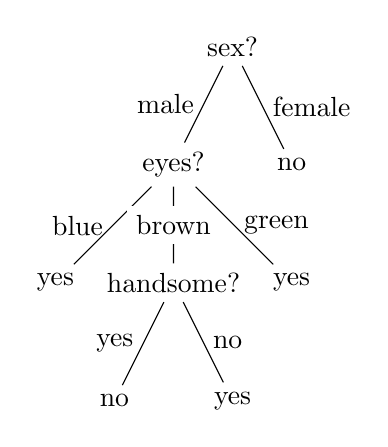
\begin{tikzpicture}
  \node {sex?}
  child { node {eyes?}
    child { node {yes} edge from parent node[left] {blue} }
    child { node {handsome?}
      child { node {no} edge from parent node[left] {yes} }
      child { node {yes} edge from parent node[right] {no} }
      edge from parent node[fill=white] {brown} }
    child { node {yes} edge from parent node[right] {green} }
    edge from parent node[left] {male} }
  child { node {no} 
    edge from parent node[right] {female}
  };
\end{tikzpicture}
\caption{Decision tree for task a)}
\label{fig:tree-nosoccer}
\end{figure}

\begin{table}[h!]
  \centering
  \begin{tabular}{cccccc|c|c}
    \toprule
    person      & eyes  & handsome & height & sex    & soccer & date & tree\\
    \midrule
    Jimbo       & blue  & no       & tall   & male   & no     & yes & yes\\
    Krusty      & green & yes      & short  & male   & yes    & no  & yes\\
    Lisa        & blue  & yes      & tall   & female & no     & no  & no\\
    Moe         & brown & no       & short  & male   & no     & no  & yes\\
    Ned         & brown & yes      & short  & male   & no     & yes & no\\
    Quimby      & blue  & no       & tall   & male   & no     & yes & yes\\
    \bottomrule
  \end{tabular}
  \caption{Classification result for tree a) on the test set. Accuracy is 3/6.}
\label{tab:tree-nosoccer}
\end{table}


\subsection{Without attribute ``eyecolor''}

The decision tree is shown in Figure~\ref{fig:tree-noeyes}.
Classification results are in Table~\ref{tab:tree-noeyes}.

\begin{figure}
\centering 
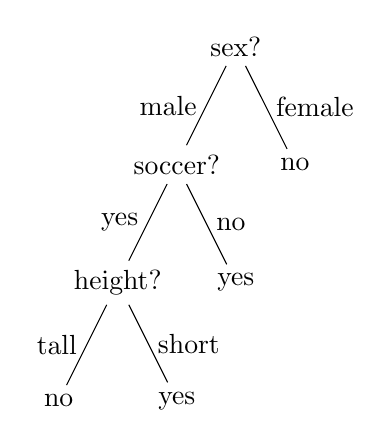
\begin{tikzpicture}
  \node {sex?}
  child { node {soccer?}
    child { node {height?}
    child { node {no} edge from parent node[left] {tall} }
    child { node {yes} edge from parent node[right] {short} }
      edge from parent node[left] {yes} }
    child { node {yes} edge from parent node[right] {no} }
    edge from parent node[left] {male} }
  child { node {no} 
    edge from parent node[right] {female}
  };
\end{tikzpicture}
\caption{Decision tree for task b)}
\label{fig:tree-noeyes}
\end{figure}

\begin{table}[h!]
  \centering
  \begin{tabular}{cccccc|c|c}
    \toprule
    person      & eyes  & handsome & height & sex    & soccer & date & tree\\
    \midrule
    Jimbo       & blue  & no       & tall   & male   & no     & yes & yes\\
    Krusty      & green & yes      & short  & male   & yes    & no  & yes\\
    Lisa        & blue  & yes      & tall   & female & no     & no  & no \\
    Moe         & brown & no       & short  & male   & no     & no  & yes\\
    Ned         & brown & yes      & short  & male   & no     & yes & yes\\
    Quimby      & blue  & no       & tall   & male   & no     & yes & yes\\
    \bottomrule
  \end{tabular}
  \caption{Classification result for tree b) on the test set. Accuracy is 4/6.}
  \label{tab:tree-noeyes}
\end{table}

\subsection{Itchy has label ``no''}

The decision tree is shown in Figure~\ref{fig:tree-itchyno}.
Classification results are in Table~\ref{tab:tree-itchyno}.

\begin{figure}
\centering 
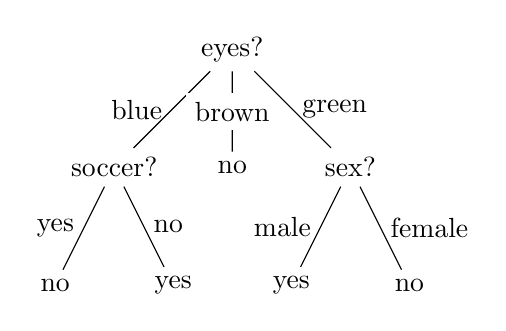
\begin{tikzpicture}
\node {eyes?}
  child { node {soccer?}
    child { node {no} edge from parent node[left] {yes} }
    child { node {yes} edge from parent node[right] {no} }
    edge from parent node[left] {blue} }
  child { node {no} edge from parent node[fill=white] {brown} }
  child { node {sex?}
    child { node {yes} edge from parent node[left] {male} }
    child { node {no} edge from parent node[right] {female} }
  edge from parent node[right] {green} }
;
\end{tikzpicture}
\caption{Decision tree for task c)}
\label{fig:tree-itchyno}
\end{figure}

\begin{table}[h!]
  \centering
  \begin{tabular}{cccccc|c|c}
    \toprule
    person      & eyes  & handsome & height & sex    & soccer & date & tree\\
    \midrule
    Jimbo       & blue  & no       & tall   & male   & no     & yes & no \\
    Krusty      & green & yes      & short  & male   & yes    & no  & yes\\
    Lisa        & blue  & yes      & tall   & female & no     & no  & yes\\
    Moe         & brown & no       & short  & male   & no     & no  & no \\
    Ned         & brown & yes      & short  & male   & no     & yes & no \\
    Quimby      & blue  & no       & tall   & male   & no     & yes & yes\\
    \bottomrule
  \end{tabular}
  \caption{Classification result for tree c) on the test set. Accuracy is 2/6.}
  \label{tab:tree-itchyno}
\end{table}

\subsection{Additional training example ``Ralph''}

The decision tree is shown in Figure~\ref{fig:tree-ralph}.
Classification results are in Table~\ref{tab:tree-ralph}.

\begin{figure}
\centering 
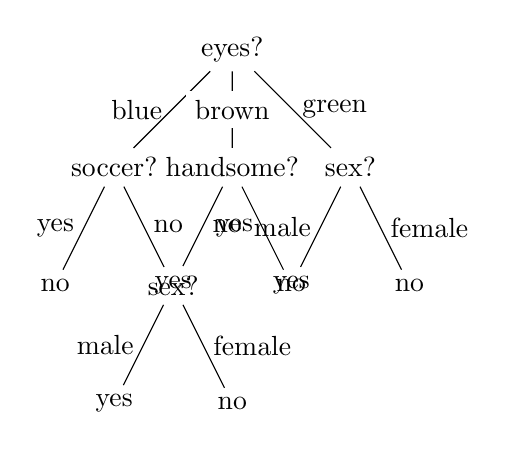
\begin{tikzpicture}
\node {eyes?}
  child { node {soccer?}
    child { node {no} edge from parent node[left] {yes} }
    child { node {yes} edge from parent node[right] {no} }
    edge from parent node[left] {blue} }
  child { node {handsome?}
    child { node {sex?}
      child { node {yes} edge from parent node[left] {male} }
      child { node {no} edge from parent node[right] {female} }
      edge from parent node[right] {no} }
    child { node {no} edge from parent node[left] {yes} }
    edge from parent node[fill=white] {brown} }
  child { node {sex?}
    child { node {yes} edge from parent node[left] {male} }
    child { node {no} edge from parent node[right] {female} }
    edge from parent node[right] {green} }
;
\end{tikzpicture}
\caption{Decision tree for task d)}
\label{fig:tree-ralph}
\end{figure}

\begin{table}[h!]
  \centering
  \begin{tabular}{cccccc|c|c}
    \toprule
    person      & eyes  & handsome & height & sex    & soccer & date & tree\\
    \midrule
    Jimbo       & blue  & no       & tall   & male   & no     & yes & yes\\
    Krusty      & green & yes      & short  & male   & yes    & no  & yes\\
    Lisa        & blue  & yes      & tall   & female & no     & no  & yes\\
    Moe         & brown & no       & short  & male   & no     & no  & yes\\
    Ned         & brown & yes      & short  & male   & no     & yes & no \\
    Quimby      & blue  & no       & tall   & male   & no     & yes & yes\\
    \bottomrule
  \end{tabular}
  \caption{Classification result for tree d) on the test set. Accuracy is 2/6.}
  \label{tab:tree-ralph}
\end{table}

